\section{GPU Programming Concepts}


\subsection{Different types of parallelism}


\subsubsection{Distributed- vs. shared-memory architecture}


\par
Most of computing problems are not trivially parallelizable, which means that the subtasks need to have access from time to time to some of the results computed by other subtasks.
The way subtasks exchange needed information depends on the available hardware.
How the information/data exchange depending on the detailed computer architecture.


\par
As shown in Fig.~\ref{fig:distributed_vs_shared}, in a distributed memory environment each computing unit operates independently from the others.
It has its own memory and it cannot access the memory in other nodes.
The communication is done via network and each computing unit runs a separate copy of the operating system.
In a shared memory machine all computing units have access to the memory and can read or modify the variables within.


\begin{figure}[!h]
\centering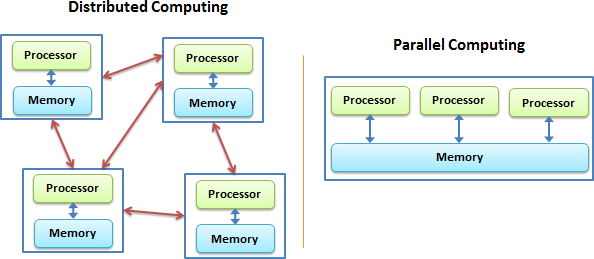
\includegraphics[width=0.8\textwidth]{fig_hardware/distributed_vs_shared.png}
\caption{Distributed- vs shared-memory parallel computing.}\label{fig:distributed_vs_shared}
\end{figure}


\subsubsection{Process-based and thread-based parallelism}


\par
The type of programming environment (distributed- or shared-memory) determines the programming model.
There are two types of parallelism,~\textbf{process-based parallelism} and~\textbf{thread-based parallelism}, as shown in Fig.~\ref{fig:process_thread_parallelism}.


\begin{figure}[!h]
\centering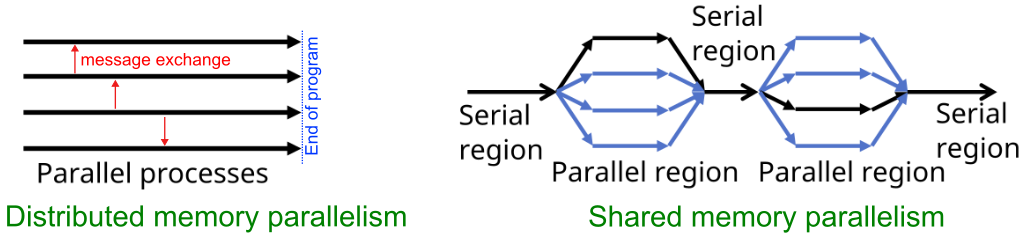
\includegraphics[width=0.8\textwidth]{fig_hardware/process_thread_parallelism.png}
\caption{The process-based and thread-based parallelism.}\label{fig:process_thread_parallelism}
\end{figure}


\par
For distributed memory machines, a process-based parallel programming model is employed.
The processes are independent execution units which have their own memory address spaces.
They are created when the parallel program is started and they are only terminated at the end.
The communication between them is done explicitly via message passing like~\textbf{MPI} (Message Passing Interface).


\par
On the shared memory architectures it is possible to use a thread-based parallelism.
The threads are light execution units and can be created and destroyed at a relatively small cost.
The threads have their own state information but they share the same memory address space.
When needed the communication is done though the shared memory.


\par
Both approaches have their advantages and disadvantages.
Distributed machines are relatively cheap to build and they have an~\lq\lq infinite\rq\rq~capacity.
In principle one could add more and more computing units.
In practice the more computing units are used the more time consuming is the communication.
The shared memory systems can achieve good performance and the programming model is quite simple.
However they are limited by the memory capacity and by the access speed.
In addition in the shared parallel model it is much easier to create race conditions.


\subsubsection{Data and task parallelism}

\par
There are two types of parallelism that can be explored, as shown in Fig.~\ref{fig:data_task_parallelism}.
The data parallelism is when the data can be distributed across computational units that can run in parallel.
The units process the data by applying the same or very similar operation to different data elements.
A common example is applying a blur filter to an image --- the same function is applied to all the pixels on an image.
This parallelism is natural for the GPU, where the same instruction set is executed in multiple threads.


\begin{figure}[!h]
\centering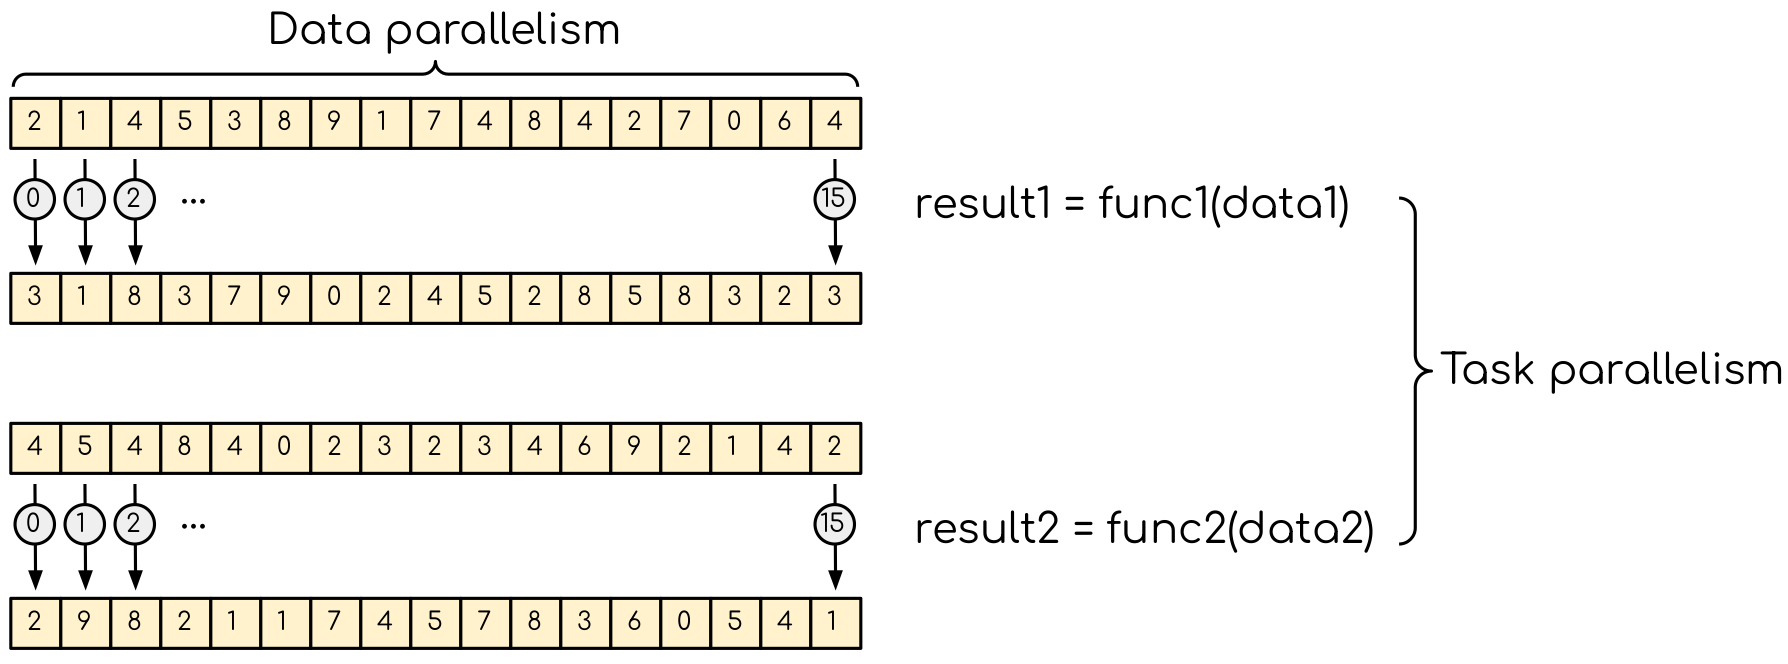
\includegraphics[width=0.8\textwidth]{fig_hardware/data_task_parallelism.png}
\caption{The data parallelism and task parallelism.}\label{fig:data_task_parallelism}
\end{figure}


\par
Data parallelism can usually be explored by the GPUs quite easily.
The most basic approach would be finding a loop over many data elements and converting it into a GPU kernel.
If the number of elements in the data set is fairly large (tens or hundred of thousands elements), the GPU should perform quite well.
Although it would be odd to expect absolute maximum performance from such a naive approach, it is often the one to take.
Getting absolute maximum out of the data parallelism requires good understanding of how GPU works.

\par
Another type of parallelism is the task parallelism.
This is when an application consists of more than one task that requiring to perform different operations with (the same or) different data.
An example of task parallelism is cooking: slicing vegetables and grilling are very different tasks and can be done at the same time.
Note that the tasks can consume totally different resources, which also can be explored.


\par
A short summary of this subsection:
\begin{itemize}
    \item Computing problems can be parallelized in distributed memory or shared memory architectures.
    \item In distributed memory, each unit operates independently, with no direct memory access between nodes.
    \item In shared memory, units have access to the same memory and can communicate through shared variables.
    \item Parallel programming can be process-based (distributed memory) or thread-based (shared memory).
    \item Process-based parallelism uses independent processes with separate memory spaces and explicit message passing.
    \item Thread-based parallelism uses lightweight threads that share the same memory space and communicate through shared memory.
    \item Data parallelism distributes data across computational units, processing them with the same or similar operations.
    \item Task parallelism involves multiple independent tasks that perform different operations on the same or different data.
    \item Task parallelism involves executing different tasks concurrently, leveraging different resources.
\end{itemize}


% -------------------------------------------------------------------- %


\subsection{GPU execution model}


\par
In order to obtain maximum performance it is important to understand how GPUs execute the programs (Fig.~\ref{fig:cpu_gpu_highway}).
As mentioned before a CPU is a flexible device oriented towards general purpose usage.
It’s fast and versatile, designed to run operating systems and various, very different types of applications.
It has lots of features, such as better control logic, caches and cache coherence, that are not related to pure computing.
CPUs optimize the execution by trying to achieve low latency via heavy caching and branch prediction.


\begin{figure}[!h]
\centering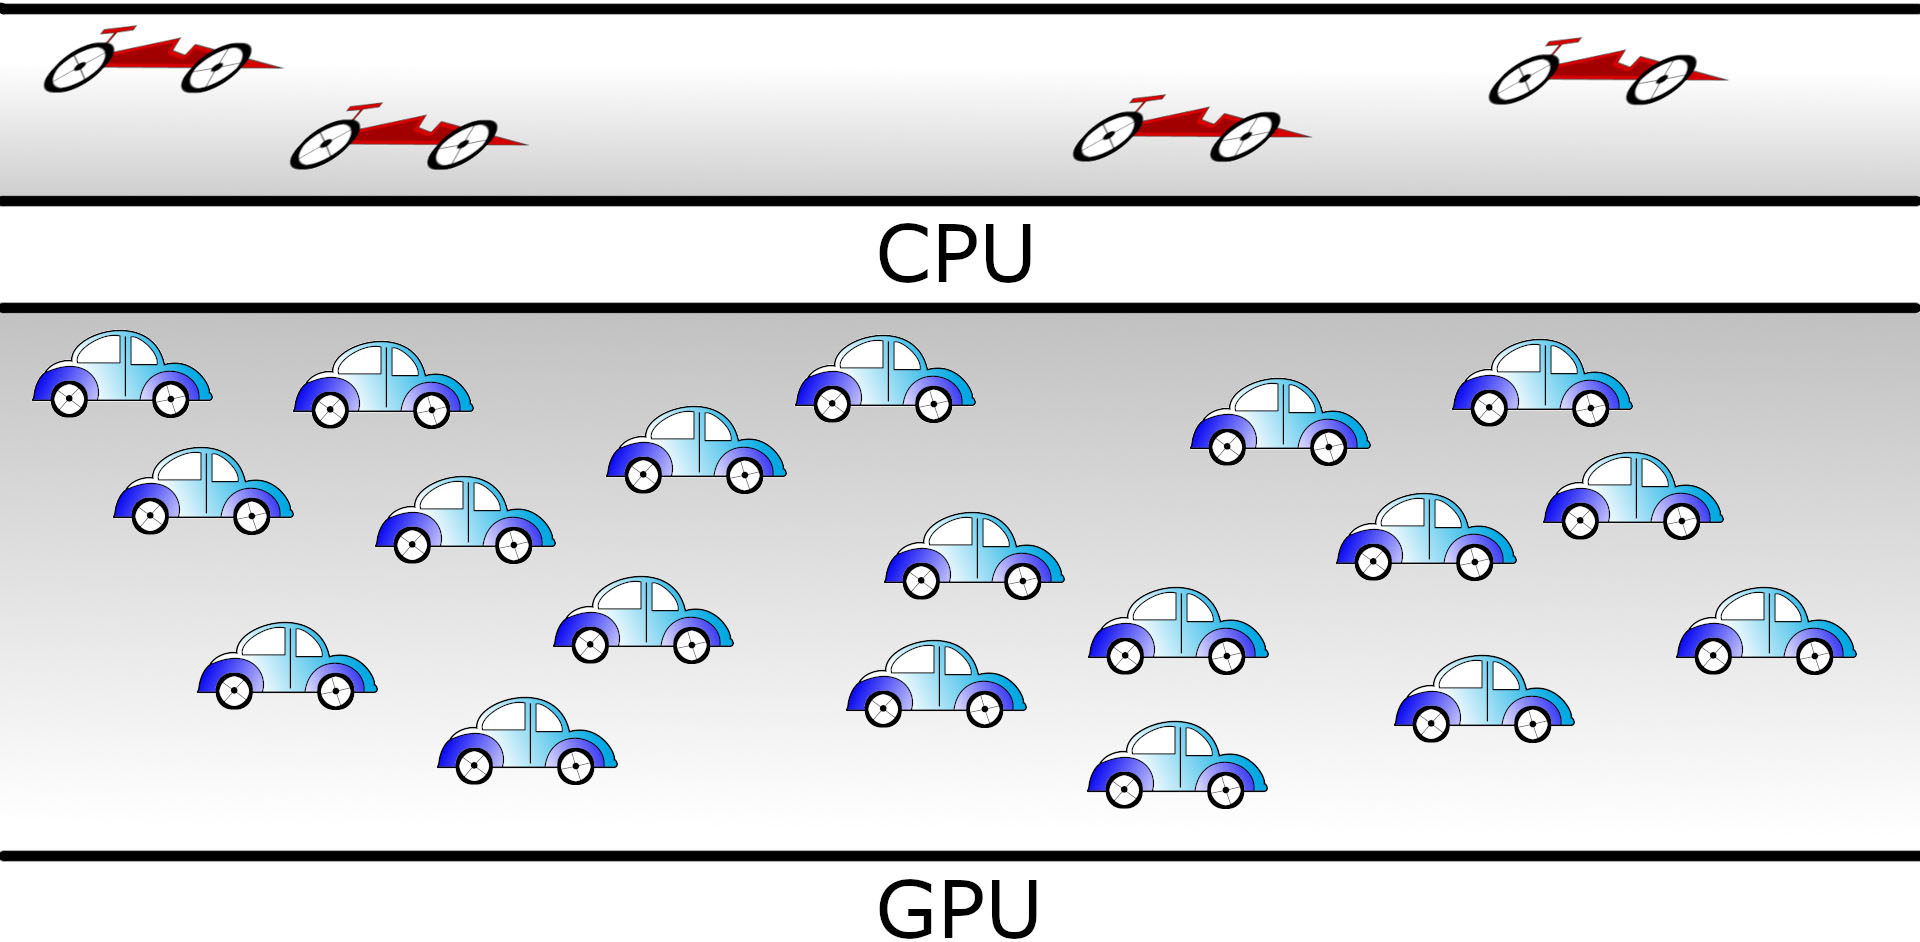
\includegraphics[width=0.8\textwidth]{fig_hardware/cpu_gpu_highway.jpg}
\caption{Cars and roads analogy for the CPU and GPU behavior. The compact road is analogous to the CPU (low latency, low throughput) and the broader road is analogous to the GPU (high latency, high throughput).}\label{fig:cpu_gpu_highway}
\end{figure}


\par
In contrast the GPUs contain a relatively small amount of transistors dedicated to control and caching, and a much larger fraction of transistors dedicated to the mathematical operations.
Since the cores in a GPU are designed just for 3D graphics, they can be made much simpler and there can be a very larger number of cores.
The current GPUs contain thousands of CUDA cores.
Performance in GPUs is obtain by having a very high degree of parallelism.
Lots of threads are launched in parallel.
For good performance there should be at least several times more than the number of CUDA cores.
GPU threads are much lighter than the usual CPU threads and they have very little penalty for context switching.
This way when some threads are performing some memory operations (reading or writing) others execute instructions.


\subsubsection{GPU threads}


\par
In order to perform some work the program launches a function called~\textbf{kernel}, which is executed simultaneously by tens of thousands of threads that can be run on GPU cores parallelly, as shown in Fig.~\ref{fig:thread_core}.
GPU threads are much lighter than the usual CPU threads and they have very little penalty for context switching.
By~\lq\lq over-subscribing\rq\rq~the GPU there are threads that are performing some memory operations (reading or writing), while others execute instructions.


\begin{figure}[!h]
\centering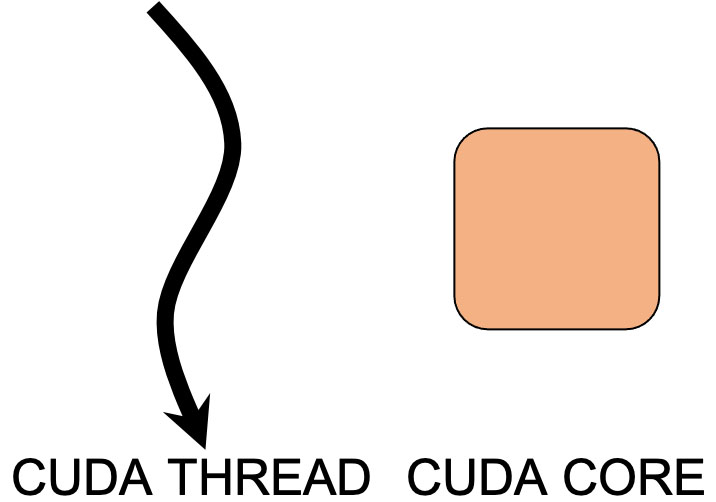
\includegraphics[width=0.5\textwidth]{fig_hardware/thread_core.jpg}
\caption{GPU Threads are executed on GPU cores}\label{fig:thread_core}
\end{figure}


\par
Every thread is associated with a particular intrinsic index which can be used to calculate and access memory locations in an array. 
Each thread has its context and set of private variables.
All threads have access to the global GPU memory, but there is no general way to synchronize when executing a kernel.
If some threads need data from the global memory which was modified by other threads the code would have to be splitted in several kernels because only at the completion of a kernel it is ensured that the writing to the global memory was completed.


\subsubsection{GPU warps}


\par
Apart from being much light weighted there are more differences between GPU threads and CPU threads.
GPU threads with consecutive thread indexes are bundled together in groups called~\textbf{warps}, as shown in Fig.~\ref{fig:warp_simt}.
This done at hardware level.


\begin{figure}[!h]
\centering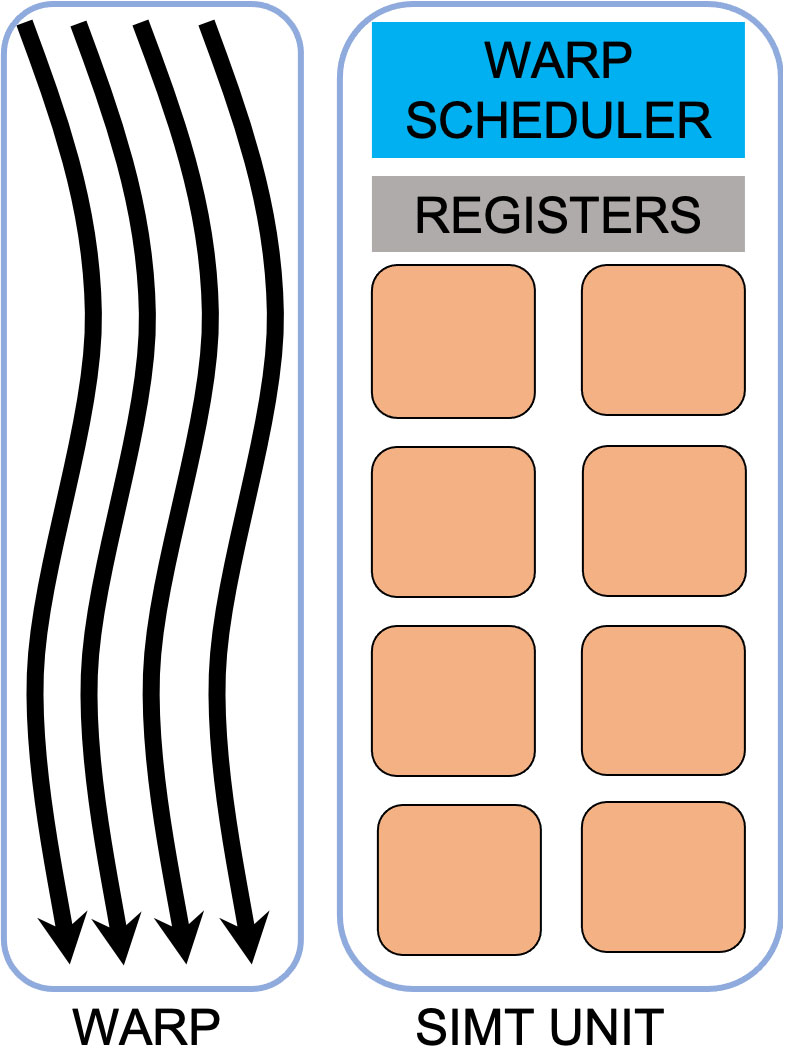
\includegraphics[width=0.4\textwidth]{fig_hardware/warp_simt.jpg}
\caption{Warp is the scheduling unit in SMs, and it executes in a SIMD manner.}\label{fig:warp_simt}
\end{figure}


\par
All memory accesses to the GPU memory are as a group in blocks of specific sizes (32B, 64B, 128B, $etc.$).
To obtain good performance, the CUDA threads in the same warp need to access elements of the data which are adjacent in the memory. 
This is called coalesced memory access.


\par
On some architectures, all members of a warp have to execute the same instruction, the so-called~\lq\lq lock-step\rq\rq~execution. 
This is done to achieve higher performance, but there are some drawbacks.
If an $if$-$else$ statement is present inside a warp will cause the warp to be executed more than once, one time for each branch.
When different threads within a single warp take different execution paths based on a conditional statement, both branches are executed sequentially, with some threads being active while others are inactive.
On architectures without lock-step execution, such as NVIDIA Volta/Turing ($e.g.$, GeForce 16xx-series) or newer, warp divergence is less costly.


\subsubsection{GPU blocks}


\par
There is another level in the GPU threads hierarchy. The threads are grouped together in so called~\textbf{blocks}.
Each block is assigned to one Streaming Multiprocessor (SMP) unit, as illustrated in Fig.~\ref{fig:block_smp}.
A SMP contains one or more SIMT (single instruction multiple threads) units, schedulers, and very fast on-chip memory.
Some of this on-chip memory can be used in the programs, this is called~\textbf{shared memory}.
The shared memory can be used to~\lq\lq cache\rq\rq~data that is used by more than one thread, thus avoiding multiple reads from the global memory.
It can also be used to avoid memory accesses which are not efficient.
For example in a matrix transpose operation, we have two memory operations per element and only can be coalesced.
In the first step a tile of the matrix is saved read a coalesced manner in the shared memory.
After all the reads of the block are done the tile can be locally transposed (which is very fast) and then written to the destination matrix in a coalesced manner as well.
Shared memory can also be used to perform block-level reductions and similar collective operations.
All threads can be synchronized at block level.
Furthermore when the shared memory is written in order to ensure that all threads have completed the operation the synchronization is compulsory to ensure correctness of the program.


\begin{figure}[!h]
\centering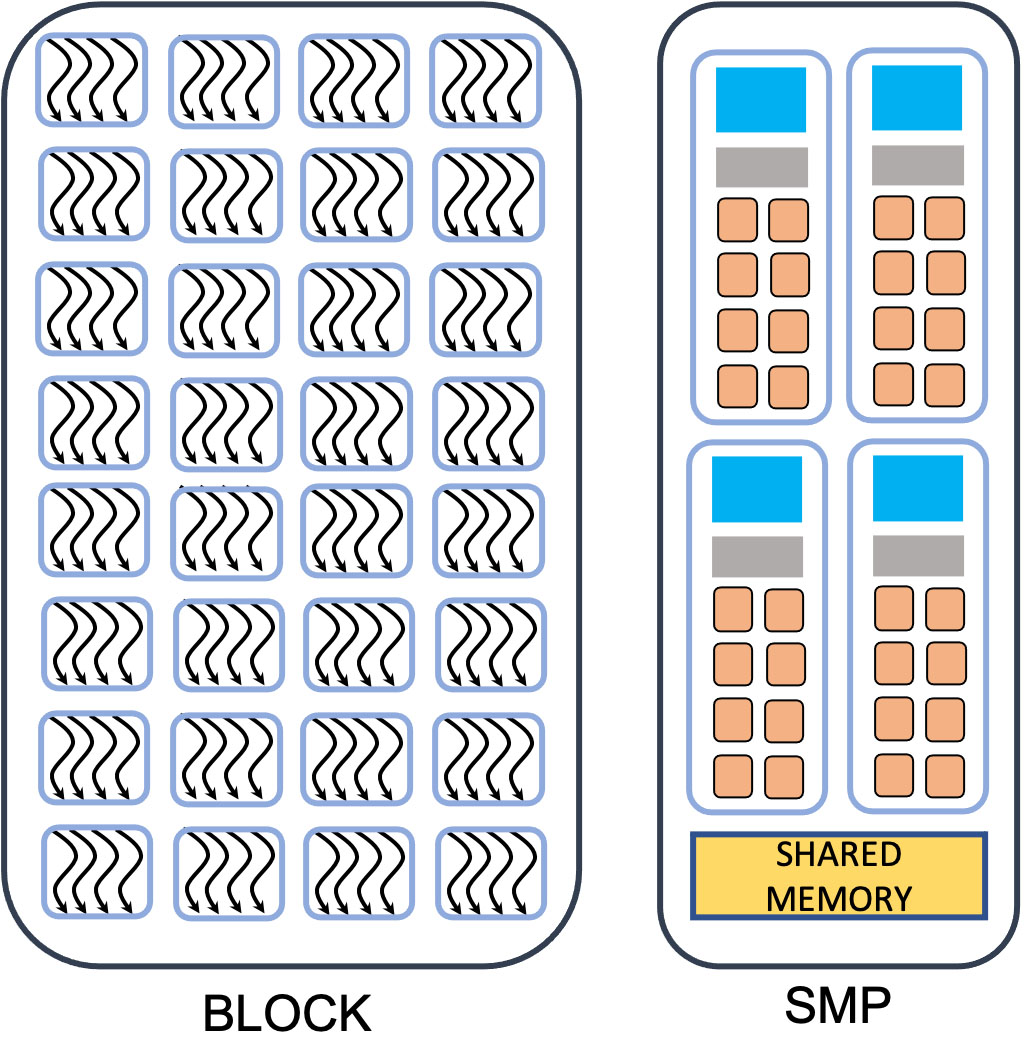
\includegraphics[width=0.5\textwidth]{fig_hardware/block_smp.jpg}
\caption{Each block is assigned to one SMP unit.}\label{fig:block_smp}
\end{figure}


\par
Finally, a block of threads can not be splitted among SMPs.
For performance blocks should have more than one warp.
The more warps are active on an SMP the better is hidden the latency associated with the memory operations.
If the resources are sufficient, due to fast context switching, an SMP can have more than one block active in the same time.
However these blocks can not share data with each other via the on-chip memory.


\par
In order to hide latencies it is recommended to~\lq\lq over-subscribe\rq\rq~the GPU.
There should be many more blocks than SMPs present on the device.
Also in order to ensure a good occupancy of the CUDA cores there should be more warps active on a given SMP than SIMT units.
This way while some warps of threads are idle waiting for some memory operations to complete, others use the CUDA cores, thus ensuring a high occupancy of the GPU.


\par
In addition to this there are some architecture-specific features of which the developers can take advantage.
Warp-level operations are primitives provided by the GPU architecture to allow for efficient communication and synchronization within a warp.
They allow threads within a warp to exchange data efficiently, without the need for explicit synchronization.
These warp-level operations, combined with the organization of threads into blocks and clusters, make it possible to implement complex algorithms and achieve high performance on the GPU.
The cooperative groups feature introduced in recent versions of CUDA provides even finer-grained control over thread execution, allowing for even more efficient processing by giving more flexibility to the thread hierarchy. Cooperative groups allow threads within a block to organize themselves into smaller groups, called cooperative groups, and to synchronize their execution and share data within the group.


\subsubsection{Mapping thread and thread block to elements of an array}


\par
In CUDA, a grid refers to the collection of thread blocks that together form the entire set of parallel work to be executed on a GPU. 
A CUDA grid is organized in a one-, two-, or three-dimensional structure, depending on the problem and data organization.
The dimensions of the grid determine how the blocks are arranged in the grid.
For example, a one-dimensional grid has a linear arrangement of blocks, while a two-dimensional grid forms a grid-like structure with rows and columns of blocks.


\par
Within a grid, individual blocks are organized in a one-, two-, or three-dimensional arrangement as well.
Each block consists of multiple threads that execute concurrently.
The dimensions of a block determine how threads are arranged within the block.
A one-dimensional block has threads arranged linearly, while a two-dimensional block has a grid-like arrangement of threads.


\par
To execute a grid of threads on the GPU, a CUDA kernel function is launched.
The kernel function defines the code that will be executed by each thread within the grid.
When launching a CUDA kernel, the size of the grid (the number of blocks) and the size of each block (the number of threads) should be clearly specified.
Within the kernel function, each thread can determine its unique index within the grid using built-in variables provided by CUDA.
For example, the variables $threadIdx.x$, $threadIdx.y$, and $threadIdx.z$ represent the thread's index within its block, while $blockIdx.x$, $blockIdx.y$, and $blockIdx.z$ represent the block's index within the grid.
The combination of these indices allows each thread to compute its unique global index within the entire grid.


\par
Fig.~\ref{fig:thread_block_index} presents an example of how the threads in a grid can be associated with specific elements of an array.
The thread marked by orange color is part of a grid of threads size 4096.
The threads are grouped in blocks of size 256.
The~\lq\lq orange\rq\rq~thread has index 3 in the block 2 and the global calculated index 515.
For a vector addition example this would be used as follow $c[index] = a[index] + b[index]$.


\begin{figure}[htbp]
\centering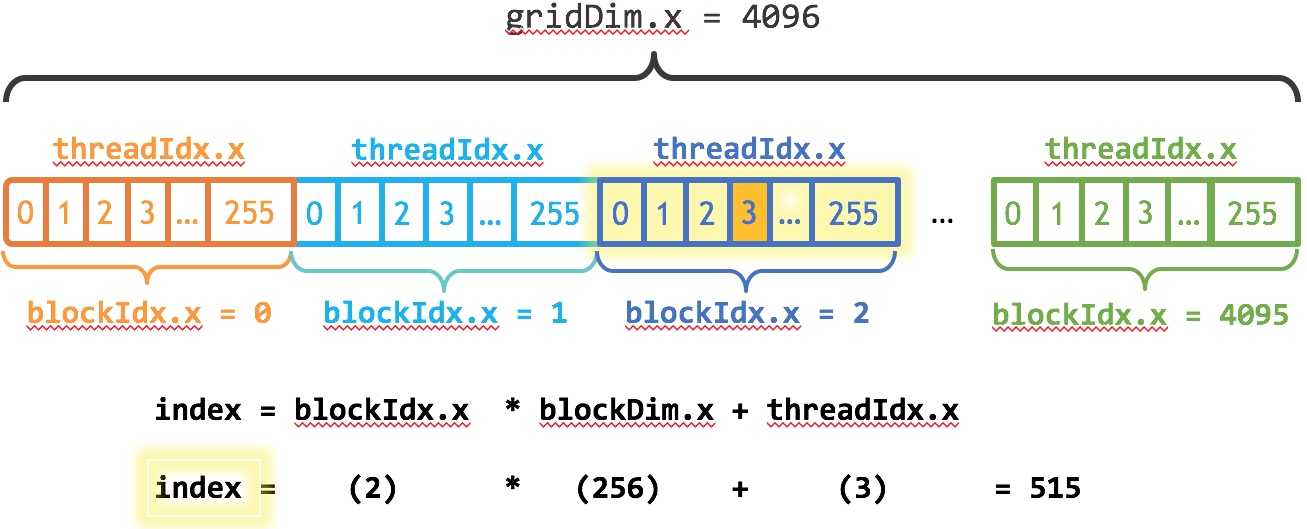
\includegraphics[width=0.8\textwidth]{fig_hardware/thread_block_index.png}
\caption{An example of the CUDA Indexing Pattern. $gridDim.x$ is the number of blocks, $blockDim.x$ is the number of threads in each block, $blockIdx.x$ is the index of the current block within the grid, and $threadIdx.x$ is the index of the current thread inside the block~\cite{indexing}.}\label{fig:thread_block_index}
\end{figure}


\par
To summarize this section.
\begin{itemize}
    \item GPUs have a distinct execution model compared to CPUs, with a focus on parallelism and mathematical operations.
    \item GPUs consist of thousands of lightweight threads that can be executed simultaneously on GPU cores.
    \item Threads are organized into warps, and warps are grouped into blocks assigned to streaming multiprocessors (SMPs).
    \item GPUs achieve performance through high degrees of parallelism and efficient memory access.
    \item Shared memory can be used to cache data and improve memory access efficiency within a block.
    \item Synchronization and data sharing are limited to the block level, with some possible sharing at the warp level depending on the architecture.
    \item Over-subscribing the GPU and maximizing warp and block occupancy help hide latencies and improve performance.
    \item Warp-level operations and cooperative groups provide efficient communication and synchronization within a warp or block.
    \item Thread indexing allows associating threads with specific elements in an array for parallel processing.
\end{itemize}


% -------------------------------------------------------------------- %


\subsection{GPU Terminology}


\par
At the moment there are three major GPU producers: NVIDIA, Intel, and AMD.
While the basic concept behind GPUs is pretty similar they use different names for the various parts.
Furthermore there are software environments for GPU programming, some from the producers and some from external groups all having different naming as well.
In Table~\ref{tbl:gpu_terminology_cuda_hip_opencl_sycl}, there is a short compilation of the some terms used across different platforms and software environments.


\begin{table}[h]
\begin{center}
\begin{threeparttable}\caption{Software mapping naming.}\label{tbl:gpu_terminology_cuda_hip_opencl_sycl}
\begin{tabular}{ |c@{\quad}|c@{\quad}|c@{\quad}|c@{\quad}| } 
\hline
\textbf{CUDA} & \textbf{HIP} & \textbf{OpenCL} & \textbf{SYCL} \\
\hline
\multicolumn{2}{|c|}{grid of threads} & \multicolumn{2}{c|}{NDRange} \\ \hline
\multicolumn{2}{|c|}{block} & \multicolumn{2}{c|}{work-group} \\ \hline
warp & wavefront & \multicolumn{2}{c|}{sub-group} \\ \hline
\multicolumn{2}{|c|}{thread} & \multicolumn{2}{|c|}{work-item} \\ \hline
\multicolumn{2}{|c|}{registers} & \multicolumn{2}{|c|}{private memory} \\ \hline
shared memory & local data share & \multicolumn{2}{|c|}{local memory} \\ \hline
\multicolumn{2}{|c|}{threadIdx.\{x,y,z\}} & get\_local\_id({0,1,2}) & nd\_item::get\_local({2,1,0})\tnote{**} \\ \hline
\multicolumn{2}{|c|}{blockIdx.{x,y,z}} & get\_group\_id({0,1,2}) & nd\_item::get\_group({2,1,0})\tnote{**} \\ \hline
\multicolumn{2}{|c|}{blockDim.{x,y,z}} & get\_local\_size({0,1,2}) & nd\_item::get\_local\_range({2,1,0})\tnote{**} \\
\hline
\end{tabular}
\begin{tablenotes}
\item[**] (1,2,3) In SYCL, the thread indexing is inverted. In a 3D grid, physically adjacent threads have consecutive X(0) index in CUDA, HIP, and OpenCL, but consecutive Z(2) index in SYCL. In a 2D grid, CUDA, HIP, and OpenCL still has contiguous indexing along X(0) dimension, while in SYCL it is Y(1). Same applies to block dimensions and indexing.
\end{tablenotes}
\end{threeparttable}
\end{center}
\end{table}

